\documentclass[screen, aspectratio=43]{beamer}
\usepackage[T1]{fontenc}
\usepackage[utf8]{inputenc}

% Use the NTNU-temaet for beamer 
% \usetheme[style=ntnu|simple|vertical|horizontal, 
%     language=bm|nn|en, 
%     smalltitle, 
%     city=all|trondheim|alesund|gjovik]{ntnu2017}
\usetheme[style=ntnu,language=en]{ntnu2017}

\usepackage[english]{babel}
\usepackage[style=numeric,backend=biber,natbib=false,sorting=none]{biblatex}

\title[PCW-d1]{Physical Computing Workshop: Day 2}
\subtitle{Sensors and actuators in our pockets}
\author[A. Xamb{\'o}]{Anna Xamb{\'o}}
\institute[NTNU]{Department of Music, NTNU}
\date{17 October 2018}
%\date{} % To have an empty date

\addbibresource{../pcw.bib} % Add bibliography database

% Set the reference style to numeric.
% See here: http://tex.stackexchange.com/questions/68080/beamer-bibliography-icon
\setbeamertemplate{bibliography item}[text] 

% Set bibliography fonts to a small size.
\renewcommand*{\bibfont}{\footnotesize}

\begin{document}

\begin{frame}
  \titlepage
\end{frame}
%
\begin{frame}
  \frametitle{Learning Outcomes}
  \begin{itemize}
    \item Identify the basic differences between sensors and actuators.
    \item Get a sense of how sensor data works in mobile phones.
    \item Be able to normalize sensor data.
    \item Explore mappings from sensor data to sound.
    \item Discern the fundamental properties of gestural interaction.   
    \item Get familiar with web technologies (Handwaving.js) and web audio technologies (Tone.js, Flocking.js).
    \item Be able to adapt javascript code of a gesture-driven musical piece with custom sounds.     
    \item Demonstrate a custom-made musical instrument in a performance setting.
    \item Reflect on the custom-made musical instrument and performance using a blogging style.   
  \end{itemize}
\end{frame}
%
\begin{frame}
  \frametitle{Preparation: Reading}
        \begin{itemize}
        \item Read / skim through the following article and be ready to discuss it in class:
         \begin{itemize}
         \item Essl, G. and Rohs, M., 2009. Interactivity for mobile music-making. Organised Sound, 14(2), pp.197-207~\cite{Essl.Rohs.2009.interactivity}:\\
         \url{https://cpb-us-w2.wpmucdn.com/people.uwm.edu/dist/0/236/files/2016/09/os09-mobileinteractivity-2lt8a0i.pdf}
         \end{itemize}    
         \end{itemize}
\end{frame}
%
\begin{frame}
  \frametitle{Preparation: What to Bring to Class?}
        \begin{itemize}
        \item Your own mobile phone (it should be a smartphone).
        \item Your own laptop.
        \item Headphones / earplugs.
         \end{itemize}
\end{frame}
%
\begin{frame}
  \frametitle{Preparation: What We Do Provide?}
        \begin{itemize}
        \item 7 Music Angel speakers for the performance per site.
        \item Slides: \url{https://github.com/axambo/physical-computing-workshop/blob/master/slides/03-d2/pcw-d2.pdf}.
        \item Code: \url{https://github.com/axambo/physical-computing-workshop/tree/master/exercises/03-d2}.
        \item A handout: \url{https://github.com/axambo/physical-computing-workshop/blob/master/handouts/pcw-d2-handout.pdf}.        
         \end{itemize}
\end{frame}
%
\begin{frame}
  \frametitle{Pre-knowledge Activity: Mobile Music}
  Be ready to discuss topics related to mobile music from the suggested reading.
\end{frame}
%
\begin{frame}
  \frametitle{Outline}
      \begin{itemize}
	\item Block I: Getting familiar with sensor data from your mobile phone
	\item Block II: Basic interactive behavior activities: mappings from sensor data to sound using gestural interaction
	\item Block III: Rehearsal and performance
    \end{itemize}  
\end{frame}
%
\begin{frame}
  \frametitle{Exercise 1: Sensor test}
     \begin{figure}
	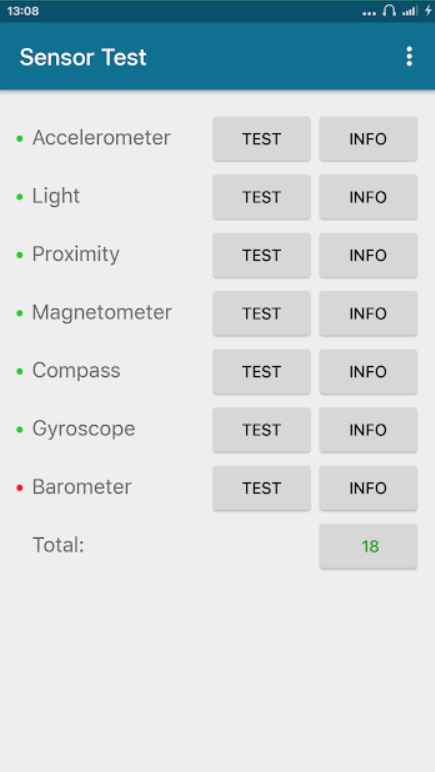
\includegraphics[scale=0.09]{img/sensor-test.png}
      \end{figure}
  {\scriptsize Most smartphones have built-in sensors that measure motion, orientation, and environmental conditions.
    \begin{itemize}
    	\item Install two mobile apps that measure sensor data of your mobile phone and compare them: what are the similarities and differences? % e.g. Sensor Test, Sensors Toolbox, Sensor Box
	\item Compare the sensors between the mobile phones of your group members: what are the similarities and differences?
	\item Observe the units of measure for each sensor: any discoveries or surprises?
	\item How would you use these sensors for a sensor-based musical app? (e.g. microphone to sing, speakers to play a sound...)
	\item What sensors (and how) would you use for a gesture-based musical app?
    \end{itemize}
  }  
  {\tiny Further reading:
  \begin{itemize}
  	\item Sensors overview (Android): \\ \url{https://developer.android.com/guide/topics/sensors/sensors_overview}
	\item Sensors overview (iPhone): \\ \url{https://developer.apple.com/documentation/coremotion}
	\item Accelerometer vs. Gyroscope: What's the Difference?: \\ \url{https://www.livescience.com/40103-accelerometer-vs-gyroscope.html}
  \end{itemize}
  }
\end{frame}
%
\begin{frame}
  \frametitle{Exercise 2: Accelerometer test in JavaScript}
       \begin{figure}
	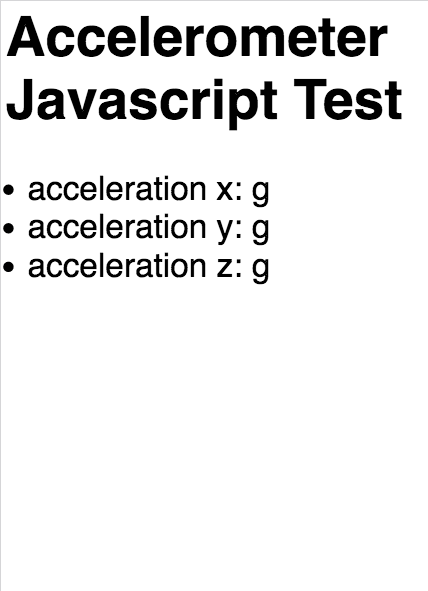
\includegraphics[scale=0.13]{img/js-accelerometer.png}
      \end{figure}
  {\scriptsize Modern browsers now support direct access to the accelerometer. The \emph{devicemotion} event is fired at a regular interval and indicates the amount of physical force of acceleration the device is receiving at that time.
    \begin{itemize}
    	\item Get familiar with the code from the file ``JS\_01\_accelerometer\_API/index.html'' and compare it with the specification of the \emph{devicemotion} event: \url{https://developer.mozilla.org/en-US/docs/Web/Events/devicemotion} -- To inspect the code you will need a code editor (e.g. Atom, Sublime), a local web server (e.g. \emph{Python SimpleHTTPServer}, \emph{Node http-server}), a browser in your laptop and a browser in your smartphone.
	\item What part of the code calculates the event and what part of the code prints the results? 
    \end{itemize}
    }
\end{frame}
%
\begin{frame}
  \frametitle{Exercise 3: Normalization of accelerometer data in JavaScript}
       \begin{figure}
	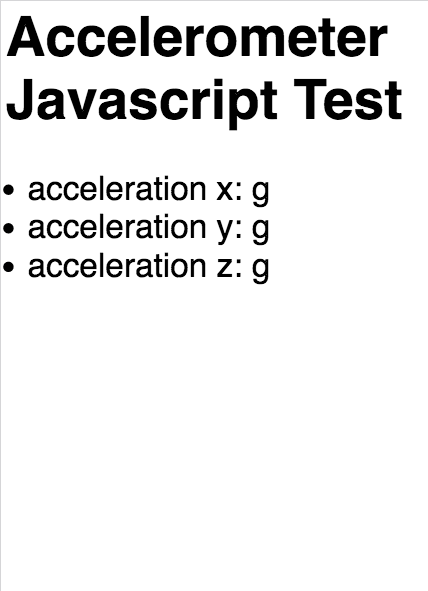
\includegraphics[scale=0.12]{img/js-accelerometer.png}
      \end{figure}
  {\scriptsize Normalization by scaling between 0 and 1 (feature scaling) is a common calculation to facilitate relations with other domains e.g. mappings to sound. The formula for normalization is:\\
  $x_{new} = \dfrac{x-x_{min}}{x_{max}-x_{min}}$
  where $x_{new}$ is the normalized value, $x_{min}$ and $x_{max}$ are the minimum and maximum values within a range. 
    \begin{itemize}
    	\item Normalize the accelerometer data from file ``JS\_02\_norm\_accelerometer\_API/index.html''. Create a function so that when you call the function you get as a result the normalized value: \\
	$x_{new}$ = \emph{normalize(x, x\_{max}, x\_{min})}
	%\item (optional) Calculate the total acceleration: $\sqrt{x^2+y^2+z^2}$\\
	%\tiny{\url{https://security.love/AccelerometerAPI/}}
    \end{itemize}
    }
\end{frame}
%
\begin{frame}
  \frametitle{Exercise 4: Handwaving}
      Handwaving is a a system for participatory mobile music based on accelerometer gesture recognition~\cite{Roma.et.al.2017.handwaving}: \url{https://github.com/g-roma/handwaving}
       \begin{figure}
	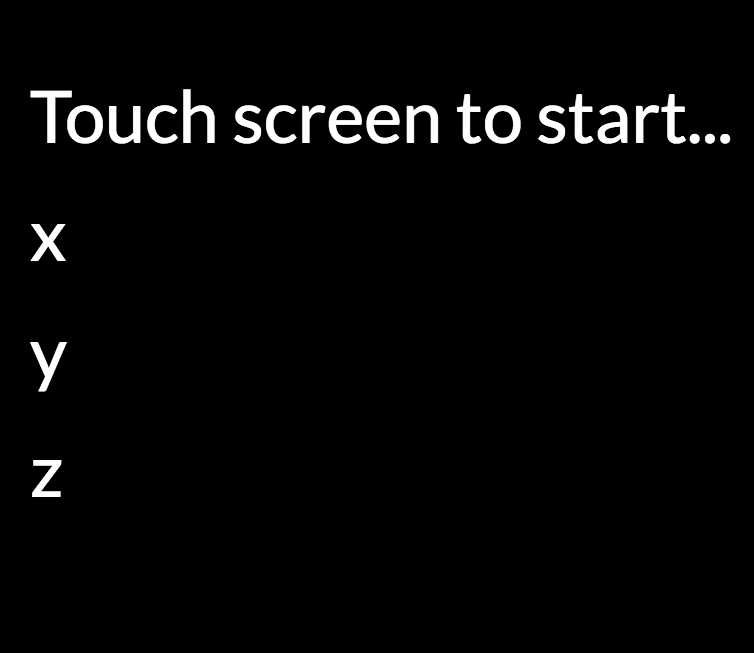
\includegraphics[scale=0.12]{img/handwaving.png}
      \end{figure}  
    \begin{itemize}
    	\item Get familiar with the code of Handwaving (\emph{HW\_01\_basic}, especially the files ``index.html'' and ``example.js'').
	\item Incorporate the code of Exercise 3 (normalization of accelerometer data) to the file (\emph{HW\_02\_normalization/example.js}).
    \end{itemize}
\end{frame}
%
\begin{frame}
  \frametitle{Exercise 5: Handwaving + Flocking.js}
  Flocking is a JavaScript audio synthesis framework: \url{http://flockingjs.org}.
    \begin{itemize}
    	\item Get familiar with the code of Handwaving + Flocking (\emph{HW\_03\_basic\_sound\_flocking}, especially \emph{function setSound()} (lines 11-21) and lines 196--238 from ``example.js'').
	\item Get familiar with the code of Handwaving + Flocking (\emph{HW\_04\_basic\_sound\_samples\_flocking}, especially \emph{function setSound()}  (lines 14--195) and lines 381--432 from ``iberlin.js'').
    \end{itemize}
\end{frame}
%
\begin{frame}
  \frametitle{Exercise 6: Handwaving + Tone.js}
  Tone.js is a framework for creating interactive music in the browser: \url{https://tonejs.github.io}
    \begin{itemize}
    	\item Explore the Tone.js library and implement it to Handwaving as the sound engine.
    \end{itemize}
\end{frame}
%
%\begin{frame}
%  \frametitle{Resources: Motion Sensors}
%    \begin{itemize}
%    	\item An Introduction to Motion Sensors: PIR, Tilt, Force, and More: \url{https://www.allaboutcircuits.com/technical-articles/an-introduction-to-motion-sensors-pir-tilt-force-and-more/}
%    \end{itemize}
%\end{frame}
%
%\begin{frame}
%  \frametitle{Resources: Normalization}
%    \begin{itemize}
%    	\item Vector magnitude & normalization: \url{https://www.khanacademy.org/computing/computer-programming/programming-natural-simulations/programming-vectors/a/vector-magnitude-normalization}
%    \end{itemize}
%\end{frame}
%
%\begin{frame}
%  \frametitle{Resources: Writing Code and Debugging in JavaScript}
%    \begin{itemize}
%    	\item Development workflow using Atom and the console from the browser
%    	\item How to view the code source
%	\item How to debug the code using the console from the browser
%    \end{itemize}
%\end{frame}
%
%\begin{frame}
%  \frametitle{Resources: Sensors in JavaScript}
%    \begin{itemize}
%    	\item Javascript Sensor API and New Browser Features Raise Privacy Concerns: \url{https://p16.praetorian.com/blog/javascript-sensor-api-new-browser-features-WebRTC-raise-privacy-concerns}
%	\item Sense and sensor-bility: access mobile device sensors with JavaScript: \url{https://mobiforge.com/design-development/sense-and-sensor-bility-access-mobile-device-sensors-with-javascript}
% 	\item Sensors For The Web!: \url{https://developers.google.com/web/updates/2017/09/sensors-for-the-web}
%    \end{itemize}
%\end{frame}
%
%\begin{frame}
%  \frametitle{Other Resources: Listening}
%    \begin{itemize}
%    	\item
%    \end{itemize}
%\end{frame}
%
\begin{frame}
  \frametitle{References}
  \printbibliography
\end{frame}

\end{document}
